
%% bare_conf.tex
%% V1.4b
%% 2015/08/26
%% by Michael Shell
%% See:
%% http://www.michaelshell.org/
%% for current contact information.
%%
%% This is a skeleton file demonstrating the use of IEEEtran.cls
%% (requires IEEEtran.cls version 1.8b or later) with an IEEE
%% conference paper.
%%
%% Support sites:
%% http://www.michaelshell.org/tex/ieeetran/
%% http://www.ctan.org/pkg/ieeetran
%% and
%% http://www.ieee.org/

%%*************************************************************************
%% Legal Notice:
%% This code is offered as-is without any warranty either expressed or
%% implied; without even the implied warranty of MERCHANTABILITY or
%% FITNESS FOR A PARTICULAR PURPOSE! 
%% User assumes all risk.
%% In no event shall the IEEE or any contributor to this code be liable for
%% any damages or losses, including, but not limited to, incidental,
%% consequential, or any other damages, resulting from the use or misuse
%% of any information contained here.
%%
%% All comments are the opinions of their respective authors and are not
%% necessarily endorsed by the IEEE.
%%
%% This work is distributed under the LaTeX Project Public License (LPPL)
%% ( http://www.latex-project.org/ ) version 1.3, and may be freely used,
%% distributed and modified. A copy of the LPPL, version 1.3, is included
%% in the base LaTeX documentation of all distributions of LaTeX released
%% 2003/12/01 or later.
%% Retain all contribution notices and credits.
%% ** Modified files should be clearly indicated as such, including  **
%% ** renaming them and changing author support contact information. **
%%*************************************************************************


% *** Authors should verify (and, if needed, correct) their LaTeX system  ***
% *** with the testflow diagnostic prior to trusting their LaTeX platform ***
% *** with production work. The IEEE's font choices and paper sizes can   ***
% *** trigger bugs that do not appear when using other class files.       ***                          ***
% The testflow support page is at:
% http://www.michaelshell.org/tex/testflow/



\documentclass[conference]{IEEEtran}
% Some Computer Society conferences also require the compsoc mode option,
% but others use the standard conference format.
%
% If IEEEtran.cls has not been installed into the LaTeX system files,
% manually specify the path to it like:
% \documentclass[conference]{../sty/IEEEtran}





% Some very useful LaTeX packages include:
% (uncomment the ones you want to load)


% *** MISC UTILITY PACKAGES ***
%
%\usepackage{ifpdf}
% Heiko Oberdiek's ifpdf.sty is very useful if you need conditional
% compilation based on whether the output is pdf or dvi.
% usage:
% \ifpdf
%   % pdf code
% \else
%   % dvi code
% \fi
% The latest version of ifpdf.sty can be obtained from:
% http://www.ctan.org/pkg/ifpdf
% Also, note that IEEEtran.cls V1.7 and later provides a builtin
% \ifCLASSINFOpdf conditional that works the same way.
% When switching from latex to pdflatex and vice-versa, the compiler may
% have to be run twice to clear warning/error messages.






% *** CITATION PACKAGES ***
%
%\usepackage{cite}
% cite.sty was written by Donald Arseneau
% V1.6 and later of IEEEtran pre-defines the format of the cite.sty package
% \cite{} output to follow that of the IEEE. Loading the cite package will
% result in citation numbers being automatically sorted and properly
% "compressed/ranged". e.g., [1], [9], [2], [7], [5], [6] without using
% cite.sty will become [1], [2], [5]--[7], [9] using cite.sty. cite.sty's
% \cite will automatically add leading space, if needed. Use cite.sty's
% noadjust option (cite.sty V3.8 and later) if you want to turn this off
% such as if a citation ever needs to be enclosed in parenthesis.
% cite.sty is already installed on most LaTeX systems. Be sure and use
% version 5.0 (2009-03-20) and later if using hyperref.sty.
% The latest version can be obtained at:
% http://www.ctan.org/pkg/cite
% The documentation is contained in the cite.sty file itself.



\usepackage{amsmath}
\usepackage{enumitem}
\usepackage{steinmetz}
\usepackage{multirow}


% *** GRAPHICS RELATED PACKAGES ***
%
\ifCLASSINFOpdf
  \usepackage[pdftex]{graphicx}
  % declare the path(s) where your graphic files are
  % \graphicspath{{../pdf/}{../jpeg/}}
  % and their extensions so you won't have to specify these with
  % every instance of \includegraphics
  % \DeclareGraphicsExtensions{.pdf,.jpeg,.png}
\else
  % or other class option (dvipsone, dvipdf, if not using dvips). graphicx
  % will default to the driver specified in the system graphics.cfg if no
  % driver is specified.
  % \usepackage[dvips]{graphicx}
  % declare the path(s) where your graphic files are
  % \graphicspath{{../eps/}}
  % and their extensions so you won't have to specify these with
  % every instance of \includegraphics
  % \DeclareGraphicsExtensions{.eps}
\fi
% graphicx was written by David Carlisle and Sebastian Rahtz. It is
% required if you want graphics, photos, etc. graphicx.sty is already
% installed on most LaTeX systems. The latest version and documentation
% can be obtained at: 
% http://www.ctan.org/pkg/graphicx
% Another good source of documentation is "Using Imported Graphics in
% LaTeX2e" by Keith Reckdahl which can be found at:
% http://www.ctan.org/pkg/epslatex
%
% latex, and pdflatex in dvi mode, support graphics in encapsulated
% postscript (.eps) format. pdflatex in pdf mode supports graphics
% in .pdf, .jpeg, .png and .mps (metapost) formats. Users should ensure
% that all non-photo figures use a vector format (.eps, .pdf, .mps) and
% not a bitmapped formats (.jpeg, .png). The IEEE frowns on bitmapped formats
% which can result in "jaggedy"/blurry rendering of lines and letters as
% well as large increases in file sizes.
%
% You can find documentation about the pdfTeX application at:
% http://www.tug.org/applications/pdftex





% *** MATH PACKAGES ***
%
%\usepackage{amsmath}
% A popular package from the American Mathematical Society that provides
% many useful and powerful commands for dealing with mathematics.
%
% Note that the amsmath package sets \interdisplaylinepenalty to 10000
% thus preventing page breaks from occurring within multiline equations. Use:
%\interdisplaylinepenalty=2500
% after loading amsmath to restore such page breaks as IEEEtran.cls normally
% does. amsmath.sty is already installed on most LaTeX systems. The latest
% version and documentation can be obtained at:
% http://www.ctan.org/pkg/amsmath





% *** SPECIALIZED LIST PACKAGES ***
%
%\usepackage{algorithmic}
% algorithmic.sty was written by Peter Williams and Rogerio Brito.
% This package provides an algorithmic environment fo describing algorithms.
% You can use the algorithmic environment in-text or within a figure
% environment to provide for a floating algorithm. Do NOT use the algorithm
% floating environment provided by algorithm.sty (by the same authors) or
% algorithm2e.sty (by Christophe Fiorio) as the IEEE does not use dedicated
% algorithm float types and packages that provide these will not provide
% correct IEEE style captions. The latest version and documentation of
% algorithmic.sty can be obtained at:
% http://www.ctan.org/pkg/algorithms
% Also of interest may be the (relatively newer and more customizable)
% algorithmicx.sty package by Szasz Janos:
% http://www.ctan.org/pkg/algorithmicx




% *** ALIGNMENT PACKAGES ***
%
%\usepackage{array}
% Frank Mittelbach's and David Carlisle's array.sty patches and improves
% the standard LaTeX2e array and tabular environments to provide better
% appearance and additional user controls. As the default LaTeX2e table
% generation code is lacking to the point of almost being broken with
% respect to the quality of the end results, all users are strongly
% advised to use an enhanced (at the very least that provided by array.sty)
% set of table tools. array.sty is already installed on most systems. The
% latest version and documentation can be obtained at:
% http://www.ctan.org/pkg/array


% IEEEtran contains the IEEEeqnarray family of commands that can be used to
% generate multiline equations as well as matrices, tables, etc., of high
% quality.




% *** SUBFIGURE PACKAGES ***
%\ifCLASSOPTIONcompsoc
%  \usepackage[caption=false,font=normalsize,labelfont=sf,textfont=sf]{subfig}
%\else
%  \usepackage[caption=false,font=footnotesize]{subfig}
%\fi
% subfig.sty, written by Steven Douglas Cochran, is the modern replacement
% for subfigure.sty, the latter of which is no longer maintained and is
% incompatible with some LaTeX packages including fixltx2e. However,
% subfig.sty requires and automatically loads Axel Sommerfeldt's caption.sty
% which will override IEEEtran.cls' handling of captions and this will result
% in non-IEEE style figure/table captions. To prevent this problem, be sure
% and invoke subfig.sty's "caption=false" package option (available since
% subfig.sty version 1.3, 2005/06/28) as this is will preserve IEEEtran.cls
% handling of captions.
% Note that the Computer Society format requires a larger sans serif font
% than the serif footnote size font used in traditional IEEE formatting
% and thus the need to invoke different subfig.sty package options depending
% on whether compsoc mode has been enabled.
%
% The latest version and documentation of subfig.sty can be obtained at:
% http://www.ctan.org/pkg/subfig




% *** FLOAT PACKAGES ***
%
%\usepackage{fixltx2e}
% fixltx2e, the successor to the earlier fix2col.sty, was written by
% Frank Mittelbach and David Carlisle. This package corrects a few problems
% in the LaTeX2e kernel, the most notable of which is that in current
% LaTeX2e releases, the ordering of single and double column floats is not
% guaranteed to be preserved. Thus, an unpatched LaTeX2e can allow a
% single column figure to be placed prior to an earlier double column
% figure.
% Be aware that LaTeX2e kernels dated 2015 and later have fixltx2e.sty's
% corrections already built into the system in which case a warning will
% be issued if an attempt is made to load fixltx2e.sty as it is no longer
% needed.
% The latest version and documentation can be found at:
% http://www.ctan.org/pkg/fixltx2e


%\usepackage{stfloats}
% stfloats.sty was written by Sigitas Tolusis. This package gives LaTeX2e
% the ability to do double column floats at the bottom of the page as well
% as the top. (e.g., "\begin{figure*}[!b]" is not normally possible in
% LaTeX2e). It also provides a command:
%\fnbelowfloat
% to enable the placement of footnotes below bottom floats (the standard
% LaTeX2e kernel puts them above bottom floats). This is an invasive package
% which rewrites many portions of the LaTeX2e float routines. It may not work
% with other packages that modify the LaTeX2e float routines. The latest
% version and documentation can be obtained at:
% http://www.ctan.org/pkg/stfloats
% Do not use the stfloats baselinefloat ability as the IEEE does not allow
% \baselineskip to stretch. Authors submitting work to the IEEE should note
% that the IEEE rarely uses double column equations and that authors should try
% to avoid such use. Do not be tempted to use the cuted.sty or midfloat.sty
% packages (also by Sigitas Tolusis) as the IEEE does not format its papers in
% such ways.
% Do not attempt to use stfloats with fixltx2e as they are incompatible.
% Instead, use Morten Hogholm'a dblfloatfix which combines the features
% of both fixltx2e and stfloats:
%
% \usepackage{dblfloatfix}
% The latest version can be found at:
% http://www.ctan.org/pkg/dblfloatfix




% *** PDF, URL AND HYPERLINK PACKAGES ***
%
%\usepackage{url}
% url.sty was written by Donald Arseneau. It provides better support for
% handling and breaking URLs. url.sty is already installed on most LaTeX
% systems. The latest version and documentation can be obtained at:
% http://www.ctan.org/pkg/url
% Basically, \url{my_url_here}.




% *** Do not adjust lengths that control margins, column widths, etc. ***
% *** Do not use packages that alter fonts (such as pslatex).         ***
% There should be no need to do such things with IEEEtran.cls V1.6 and later.
% (Unless specifically asked to do so by the journal or conference you plan
% to submit to, of course. )


% correct bad hyphenation here
\hyphenation{op-tical net-works semi-conduc-tor}


\begin{document}
%
% paper title
% Titles are generally capitalized except for words such as a, an, and, as,
% at, but, by, for, in, nor, of, on, or, the, to and up, which are usually
% not capitalized unless they are the first or last word of the title.
% Linebreaks \\ can be used within to get better formatting as desired.
% Do not put math or special symbols in the title.
\title{Comparison of Digital Demodulation Algorithms for LVDT Sensors in Circuits with Lightning Protection}
%\title{Comparison of Digital Demodulation\\Algorithms for LVDT Sensors}

% author names and affiliations
% use a multiple column layout for up to three different
% affiliations
\author{\IEEEauthorblockN{Marcos A. O. Campos Filho, MC}
\IEEEauthorblockA{Instituto Tecnol\'{o}gico de Aeron\'{a}utica\\marcos.filho@embraer.com.br}
\and
\IEEEauthorblockN{Prof. Luiz Carlos Sandoval G\'{o}es}
\IEEEauthorblockA{Instituto Tecnol\'{o}gico de Aeron\'{a}utica\\goes@ita.br}
\and
\IEEEauthorblockN{Raphael das Neves Calvo, MC}
\IEEEauthorblockA{EMBRAER\\raphael.calvo@embraer.com.br}
}

% conference papers do not typically use \thanks and this command
% is locked out in conference mode. If really needed, such as for
% the acknowledgment of grants, issue a \IEEEoverridecommandlockouts
% after \documentclass

% for over three affiliations, or if they all won't fit within the width
% of the page, use this alternative format:
% 
%\author{\IEEEauthorblockN{Michael Shell\IEEEauthorrefmark{1},
%Homer Simpson\IEEEauthorrefmark{2},
%James Kirk\IEEEauthorrefmark{3}, 
%Montgomery Scott\IEEEauthorrefmark{3} and
%Eldon Tyrell\IEEEauthorrefmark{4}}
%\IEEEauthorblockA{\IEEEauthorrefmark{1}School of Electrical and Computer Engineering\\
%Georgia Institute of Technology,
%Atlanta, Georgia 30332--0250\\ Email: see http://www.michaelshell.org/contact.html}
%\IEEEauthorblockA{\IEEEauthorrefmark{2}Twentieth Century Fox, Springfield, USA\\
%Email: homer@thesimpsons.com}
%\IEEEauthorblockA{\IEEEauthorrefmark{3}Starfleet Academy, San Francisco, California 96678-2391\\
%Telephone: (800) 555--1212, Fax: (888) 555--1212}
%\IEEEauthorblockA{\IEEEauthorrefmark{4}Tyrell Inc., 123 Replicant Street, Los Angeles, California 90210--4321}}




% use for special paper notices
%\IEEEspecialpapernotice{(Invited Paper)}




% make the title area
\maketitle

% As a general rule, do not put math, special symbols or citations
% in the abstract
\begin{abstract}
The implementation of digital Control Systems can bring several advantages to aircraft manufacturers including improvement in reliability and increased tolerance to environmental conditions such as temperature and electrical noise. 

A Simulink model for a digital position acquisition system for aircraft primary control surfaces is presented, comprised by a Linear Variable Differential Transformer (LVDT) as displacement sensor, a protective passive filter for lightning induced transients, an Analog-to-Digital converter and a digital demodulation system. 

This work performs an implementation and comparison of two strategies: the Peak Detector, based on the instant amplitude of the signal and the Oversampling/Averaging, based on the mean value of the signal over a time window.

\end{abstract}

% no keywords

% For peer review papers, you can put extra information on the cover
% page as needed:
% \ifCLASSOPTIONpeerreview
% \begin{center} \bfseries EDICS Category: 3-BBND \end{center}
% \fi
%
% For peerreview papers, this IEEEtran command inserts a page break and
% creates the second title. It will be ignored for other modes.
\IEEEpeerreviewmaketitle

\section{Introduction}
% no \IEEEPARstart

%\subsection{Motivation and Objective}

The main objective of this work is to evaluate the performance of two digital algorithms, Peak Detector and Oversampling/Averaging to demodulate the output of an LVDT, utilized as positioning sensor on an electro-hydraulic actuator. The constructed position acquisition system will then be integrated to the electro-hydraulic actuator model developed in \cite{Ballesteros} and the composite model will serve as platform to analyse both strategies under the following aspects:

\begin{enumerate}
\item Steady state error for a step input;
\item Effect of number of sampled points per cycle;
\item Tolerance to noise on input.
\end{enumerate}

%\subsection{Bibliographic Review}

%\cite{nyce} presents in detail the operation of several types of linear position sensors used in industry, their performance specifications and applications. The topics about the Linear Variable Differential Transformer also cover signal conditioning and analog demodulation.

%\cite{rogeriodias} presents an electrical model of an LVDT sensor which was used to simulate and design a signal conditioning circuit and synchronous analog demodulation scheme.

%\cite{do160} defines standard environmental test conditions and procedures for airborne equipment (DO-160). The purpose of these tests is to provide a controlled (laboratory) means of assuring the performance characteristics of airborne equipment in environmental conditions similar of those which may be encountered in airborne operation of the equipment. Specifically, Section 22 (Lightning Induced Transient Susceptibility) provides the specific guidelines for testing the resilience of an equipment against indirect lightning effects.

%\cite{daqhandbook}, \cite{slaa013}, \cite{maximadc} and \cite{nationaladc} present in details the inner workings of analog-to-digital converters (ADCs), covering the modern architectures with their advantages and limitations, the non-idealities inherent to these devices and how they are mitigated, in addition to pratical aspects of real-world applications.

%\cite{Constantino} develops a high fidelity model representative up to high frequencies of a Flight Control System with hydraulic actuation on active-active mode, comprised of an EHSV, hydraulic actuator, a position loop and the control surface. The step input response and frequency response were shown to be close to a real system response up to high frequencies and the behavior of an oscillatory mal-function scenario was studied, showing the expected level of structure load, as well as its fatigue life consumption.

%\cite{Ballesteros} develops a primary actuator classic sizing methodology, which is validated using an actuator model based on \cite{Constantino}. The performance for different classical controllers (P, PI, PD, and PID), in addition to modern control approaches is evaluated. The modern controllers presented good performance and enhanced the actuator's dynamic stiffness especially for frequencies above 10 Hz, allowing a piston area reduction of one seal size. It was also presented the feasibility to design an optimized flight control actuator, taking credit of a modern control approach that would reduce hydraulic consumption, and the actuator's weight and size,
%bringing benefits to the aircraft performance.

%\cite{astrom} provides a broad overview of theory and practical aspects discrete-time systems, covering the mathematical foundation, sampling theory, design and analysis of digital controllers.

\section{Model Construction}

\subsection{Linear Variable Differential Transformer}

This section presents the implementation of an 6-wire Linear Variable Differential Transformer (LVDT) model using Simscape, a library to model physical systems within the Simulink environment. The custom behavioral model is described by a system of differential algebraic equations (DAEs) and was built using Simscape language \cite{mathworks}. The LVDT is comprised of three coils within which a magnetically permeable core moves to provide variable magnetic coupling between the primary coil and the secondary coils A and B. An equivalent circuit for the LVDT is presented in Figure \ref{fig:lvdtcirc}, similar to one used by \cite{rogeriodias}.

\begin{figure}[h!]
\centering
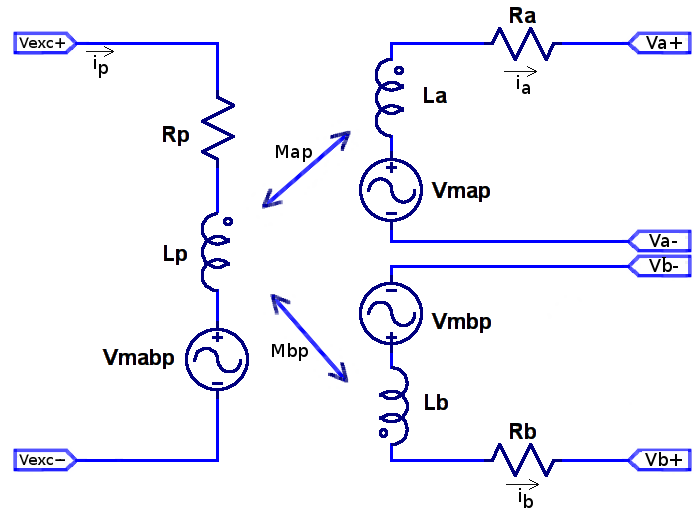
\includegraphics[scale=0.22]{pics/theory/lvdt_full_eq_circ.png}
\caption{LVDT equivalent circuit}
\label{fig:lvdtcirc}
\end{figure}
%
The values $L_k$ and $R_k$ are the self-inductance and resistance of the winding $k$ (primary or secondaries A or B). Similarly, $i_k$ denotes the current on winding $k$. $M_{ap}$ and $M_{bp}$ are the mutual inductances between the primary coil and each secondary, given by equation \ref{eq:mutind} \cite{eletrotutomutual}. 

\begin{equation}
\begin{split}
M_{ap} & = k_a(t) \sqrt{L_a L_p} \\
M_{bp} & = k_b(t) \sqrt{L_b L_p}
\end{split}
\label{eq:mutind}
\end{equation}
%
where values $k_a(t)$ and $k_b(t)$ are the {\it coupling coefficients}, varying in time. The voltages induced on each secondary are represented by $V_{map}$ and $V_{mbp}$ in Figure \ref{fig:lvdtcirc}. 

Considering two coils in the configuration shown in Figure \ref{fig:coilcoupling}, using Faraday's Law, it is possible to show that the voltage $V$ induced in coil 2 due to $I_1$ and a time-varying coupling coefficient (and in consequence a time-varying mutual inductance $M(t)$) is given by equation \ref{eq:final_equation_mut}.

\begin{equation}
V = \frac{dM(t)}{dt} I_1 + M(t) \frac{dI_1}{dt} 
\label{eq:final_equation_mut}
\end{equation}

\begin{figure}[h!]
\centering
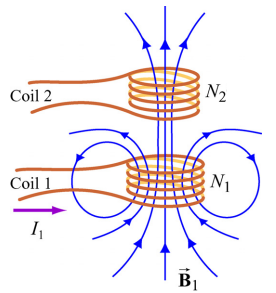
\includegraphics[scale=0.25]{pics/models/coil_coupling.png}
\caption{Coupled coils - Source \cite{coilsmut}}
\label{fig:coilcoupling}
\end{figure}

When the LVDT is totally retracted, the coupling coefficient $k_a$ is $K_{min}$ and $k_b$ is $K_{max}$ and when totally extended, the opposite. Since the variation is linear with core position $x(t)$ (normalized), the coupling coefficients can be expressed by equations \ref{eq:kakboft}.

\begin{equation}
\begin{split}
k_a(t) & = \frac{K_{max} - K_{min}}{2}x(t) + \frac{K_{max} + K_{min}}{2} \\
k_b(t) & = \frac{-(K_{max} - K_{min})}{2}x(t) + \frac{K_{max} + K_{min}}{2}
\end{split}
\label{eq:kakboft}
\end{equation}

The Simscape expression for primary and secondary windings are given by equations \ref{eq:vpriexpr} and \ref{eq:vsecexpr} respectively. Suitable values for the simulation were obtained from typical values collected from multiple sources (\cite{lvdtdatasheet1}, \cite{lvdtdatasheet2}, \cite{lvdtdatasheet3}). The parameters for the model are summarized on Table \ref{tab:lvdtparam}.

\begin{equation}
\begin{split}
V_{exc} == R_p i_p + L_p \frac{di_p}{dt} & + \left(M_{ap} \frac{di_a}{dt} + i_a \frac{dM_{ap}}{dt} \right) \\
	& + \left(M_{bp} \frac{di_b}{dt} + i_b \frac{dM_{bp}}{dt}\right)
\end{split}
\label{eq:vpriexpr}
\end{equation}

\begin{equation}
\begin{split}
V_a & == R_a i_a + L_a \frac{di_a}{dt} + \left(M_{ap} \frac{di_p}{dt} + i_p \frac{dM_{ap}}{dt}\right) \\
V_b & == R_b i_b + L_b \frac{di_b}{dt} + \left(M_{bp} \frac{di_p}{dt} + i_p \frac{dM_{bp}}{dt}\right)
\end{split}
\label{eq:vsecexpr}
\end{equation}

\begin{table}[h!]
\centering
\caption{LVDT parameters}
\label{tab:lvdtparam}
\begin{tabular}{|c|c|}
\hline
Parameter                            & Value        \\
\hline
Excitation voltage ($V_{exc}$) & $7V_{RMS}~@~3kHz$ \\ \hline
Primary inductance ($L_p$) / resistance ($R_p$) & $80mH$ / $200\Omega$ \\ \hline
Secondary A inductance ($L_a$) / resistance ($R_a$) & $40mH$ / $150\Omega$ \\ \hline
Secondary B inductance ($L_b$) / resistance ($R_b$) & $40mH$ / $150\Omega$ \\ \hline
Coupling coefficients [$K_{min}$, $K_{max}$] & [$0.178$~,~$0.535$] \\ \hline
Maximum absolute ratio (ratiometric demodulation) & $0.5$ \\ \hline
Minimum signal voltage (full extended) & $0.873 V_{RMS}$ \\ \hline
Maximum signal voltage (full extended) & $2.625 V_{RMS}$ \\ \hline
Maximum phase & $7.55^{\circ}$ \\ \hline
\end{tabular}
\end{table}


\subsection{Transient Filter}

Aircraft manufacturers refer to RTCA/DO-160 Section 22 (Lightning Induced Transient Susceptibility) \cite{do160} as minimum requirements to design and test airborne equipment with standardized and representative waveforms for lightning induced transients. For a typical configuration where the actuator is installed in a non-pressurized region and its sensor interfaces and cabling passes through non-metallic (composite) regions, a pin injection test comprised of Waveforms 3 and 4 (Figure \ref{fig:dowaveform34}) at power level 3 \cite{do160} is indicated to verify the controller's susceptibility. A passive low pass filter was designed to atenuate the waveforms so the maximum output lies below $10V$.% \cite{vishay}. 

\begin{figure}[h!]
\centering
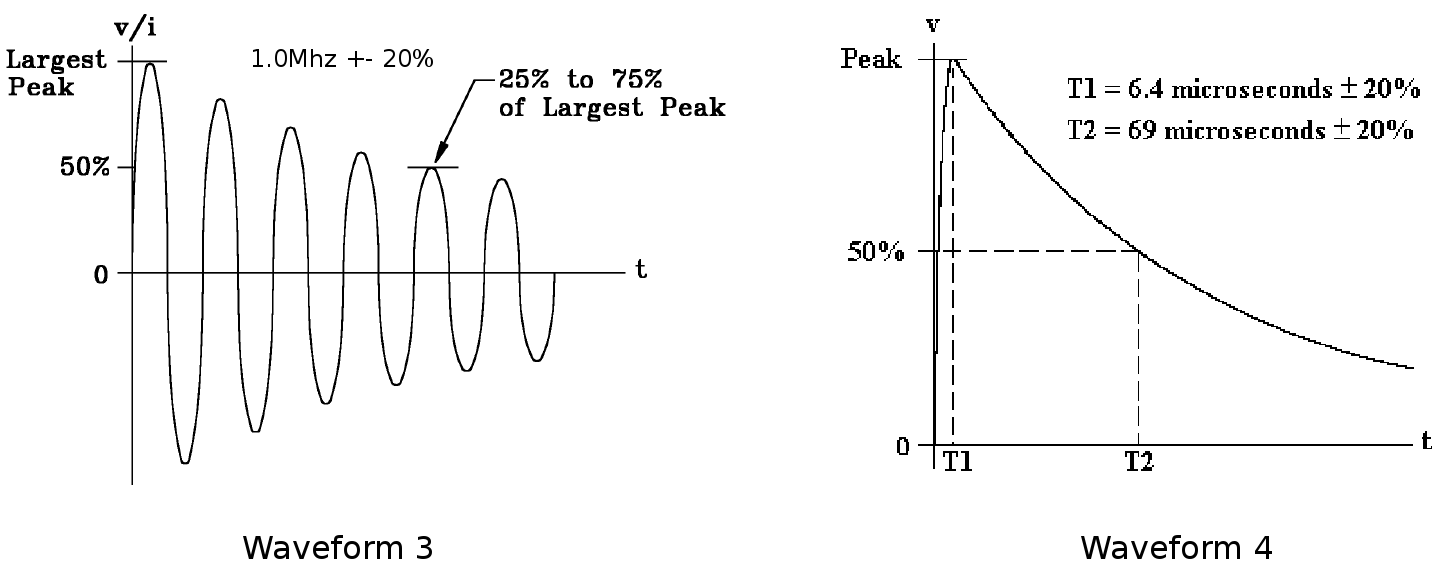
\includegraphics[scale=0.18]{pics/theory/waveforms.png}
\caption{Waveforms 3 and 4 - Source: \cite{do160}}
\label{fig:dowaveform34}
\end{figure}

%A passive low pass filter was designed to atenuate the waveforms so the maximum output lies below $10V$ \cite{vishay}. The varistors ($U_3$ and $U_4$) provide a very low resistance path to the ground when input voltage is above a determined level \cite{vishay}. Detecting and handling these transients in the controller is out of the scope of this work so to speed up the simulation a simplified RC filter with similar frequency response around $3kHz$ was used. The filter parameters are summarized in Tables \ref{tab:rcfilter123567} and \ref{tab:rcfilterwol}.

%Detecting and handling these transients in the controller is out of the scope of this work so to speed up the simulation a simplified RC filter with similar frequency response around $3kHz$ was used. The filter parameters are summarized in Tables \ref{tab:rcfilter123567} and \ref{tab:rcfilterwol}.

Detecting and handling these transients in the controller is out of the scope of this work so to speed up the simulation a simplified RC filter with similar frequency response around $3kHz$ was used, with cutoff frequency at $30kHz$. The filters parameters are summarized on Table \ref{tab:rcfilterwol}.

%\begin{figure}[h!]
%\centering
%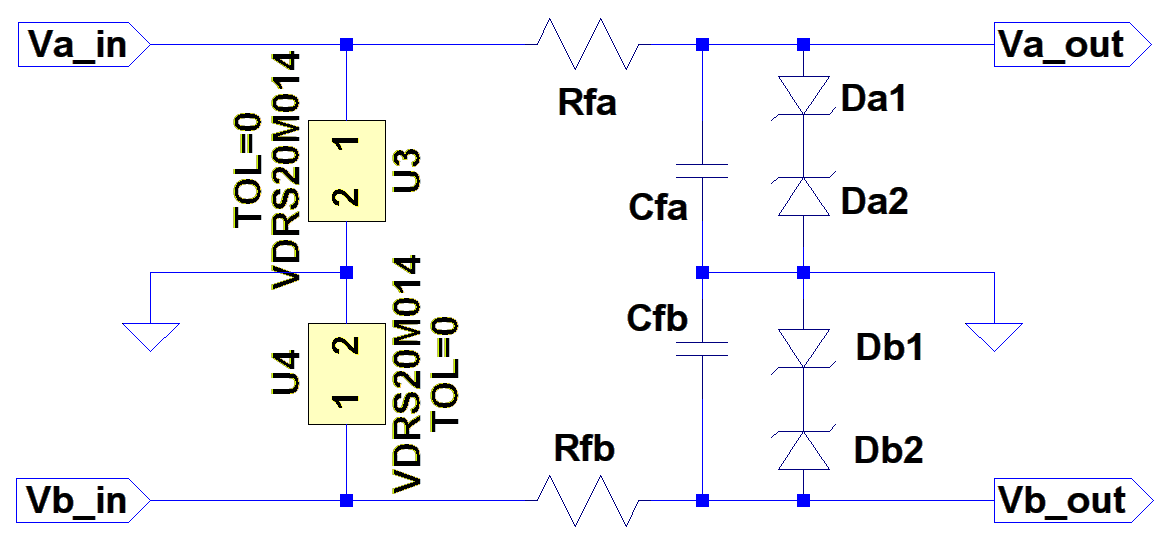
\includegraphics[scale=0.18]{pics/theory/complete_transient_filter.png}
%\caption{Complete transient filter}
%\label{fig:tranfilter}
%\end{figure}

%\begin{table}[h!]
%\centering
%\caption{RC Low pass filter parameters - I}
%\label{tab:rcfilter123567}
%\begin{tabular}{|c|c|}
%\hline
%Parameter & Value \\ \hline
%$R_f$ & $510 \Omega$ \\ \hline
%$C_f$ & $10nF$ \\ \hline
%Calculated cut-off frequency & $ 30000.00 Hz$ \\ \hline
%Real cut-off frequency & $ 31206.85 Hz$ \\ \hline
%\end{tabular}
%\end{table}	

\begin{table}[h!]
\centering
\caption{RC Low pass filter parameters}
\label{tab:rcfilterwol}
\begin{tabular}{|c|c|c|c|}
\hline
Parameter & Unfiltered & Complete filter & Simplified filter \\ \hline
Magnitude $@3kHz$ & $-8.519dB$ & $-4.549dB$ & $-7.717dB$ \\ \hline
Phase $@3kHz$ & $7.554^{\circ}$ & $-11.37^{\circ}$ & $-0.66^{\circ}$ \\ \hline
\end{tabular}
\end{table}	

\subsection{Range Converter}

This circuit is used to match the signal range of the filter output to the input of the analog-to-digital converter. This step also makes possible to balance the attenuation caused by the previous filtering stage and serves as a high impedance load for the filter and a low impedance source for the ADC. \cite{sloa097} provides guiding to design a circuit capable of adding gain and DC offset to a signal, based on the desired input and output ranges (Table \ref{tab:rangeconvfinal2}).

%\begin{figure}[h!]
%\centering
%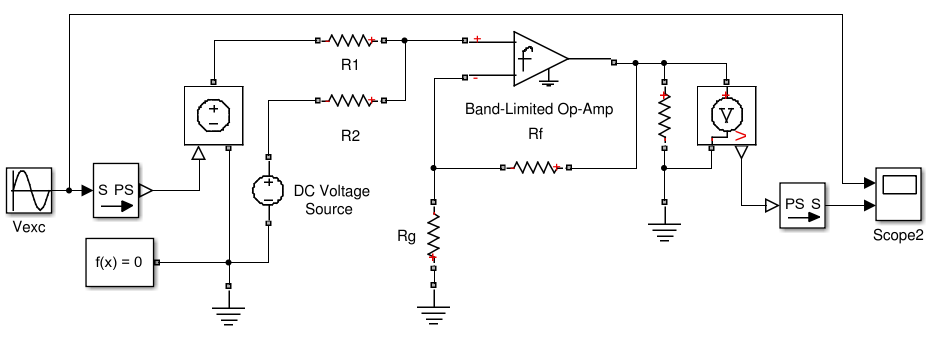
\includegraphics[scale=0.22]{pics/models/scale_offset_circuit.png}
%\caption{Gain and DC offset circuit test model}
%\label{fig:vscalecircuit}
%\end{figure}

%\begin{table}[h!]
%\centering
%\caption{Gain and DC offset circuit parameters}
%\label{tab:rangeconvparam2}
%\begin{tabular}{|c|c|}
%\hline
%Parameter & Value \\ \hline
%$R_1$ & $357k\Omega$ 			\\ \hline
%$R_2$ & $392k\Omega$ 			\\ \hline
%$R_f$ & $7.68k\Omega$		 	\\ \hline
%$R_g$ & $7.15k\Omega$		 	\\ \hline
%$V_{ref}$ & $5V$		 	\\ \hline
%OpAmp Open Loop Gain ($A$) & $10^4$ 			\\ \hline
%OpAmp Input resistance ($R_{in}$) & $1 M\Omega$ 			\\ \hline
%OpAmp Output resistance ($R_{out}$) & $100 \Omega$ 			\\ \hline
%OpAmp Minimum output ($V_{min}$) & $-12V$ 			\\ \hline
%OpAmp Maximum output ($V_{max}$) & $12V$ 			\\ \hline
%OpAmp Maximum slew rate ($\dot V$) & $10 V/us$ 			\\ \hline
%OpAmp Bandwidth ($BW$) & $100kHz$ 			\\ \hline
%\end{tabular}
%\end{table}	

\begin{table}[h!]
\centering
\caption{Range converter model parameters}
\label{tab:rangeconvfinal2}
\begin{tabular}{|c|c|}
\hline
Parameter & Value \\ \hline
Input signal range  & [-$4.50$~,$4.50$]$V$  \\ \hline
Output signal range  & [$0.02$~,$9.40$]$V$ \\ \hline
ADC range utilization & $93.8\%$ \\ \hline
\end{tabular}
\end{table}

\subsection{Analog-to-Digital Converter}

This section presents the behavioral model of a Successive Approximation Register (SAR) ADC which performance parameters were based on the Texas Instruments ADS8638, a 12-bit SAR ADC capable of measuring 8 time-multiplexed channels in multiple selectable ranges up to $\pm 10V$ at $1 MSPS$. This device provides a sample-and-hold front-end with no latency in conversions and no missing codes \cite{ads8638}. 

\subsubsection{Input Stage}

The input stage of the ADC was modelled as a voltage meter across a large value resistor ($1M\Omega$) for each input, as shown on figure \ref{fig:adcinputstage}. The settling time of the ADS8638 is in the order of $250ns$, which is considered instantaneous given the simulation step time of $100ns$. It is also assumed that the output of the multiplexer is connected to a buffer with input resistance many times larger than the conduction resistance of each channel.


\begin{figure}[h!]
\centering
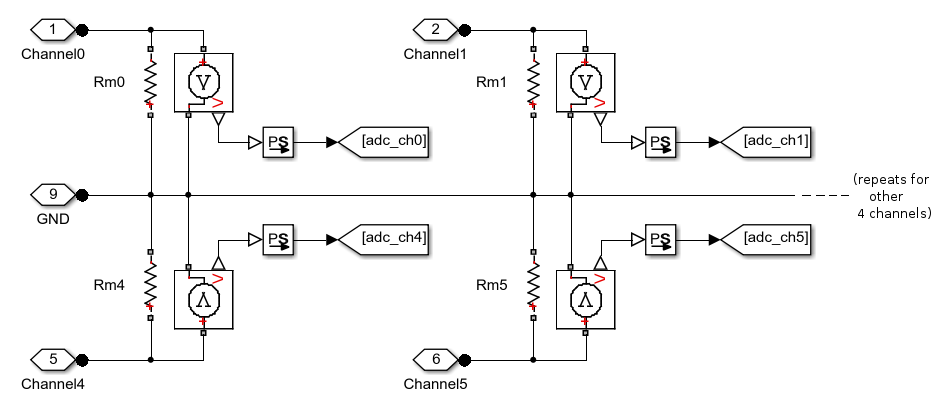
\includegraphics[scale=0.25]{pics/models/adc_input_block.png}
\caption{ADC input stage}
\label{fig:adcinputstage}
\end{figure}

\subsubsection{Channel crosstalk and channel selection}

A square matrix with order equal to the number of channels is built as shown in \ref{eq:ctmul}, where $CT_g$ is the channel crosstalk gain, extracted from datasheet. In order to simplify the implementation, it is considered that the crosstalk is the same for each pair of channels. The output is fed to a multiport switch that selects the appropriate channel.

\begin{equation}
\begin{bmatrix}
 \hat{V}_{Ch_0} \\
 \hat{V}_{Ch_1} \\
  \vdots  \\
 \hat{V}_{Ch_{n-1}} \\
 \end{bmatrix} 
=
 \begin{bmatrix}
  1 & CT_g & \cdots & CT_g \\
  CT_g & 1 & \cdots & CT_g \\
  \vdots  & \vdots  & \ddots & \vdots  \\
  CT_g & CT_g & \cdots & 1
 \end{bmatrix}
\begin{bmatrix}
 V_{Ch_0} \\
 V_{Ch_1} \\
  \vdots  \\
 V_{Ch_{n-1}} \\
 \end{bmatrix}
\label{eq:ctmul}
\end{equation}

%\begin{figure}[h!]
%\centering
%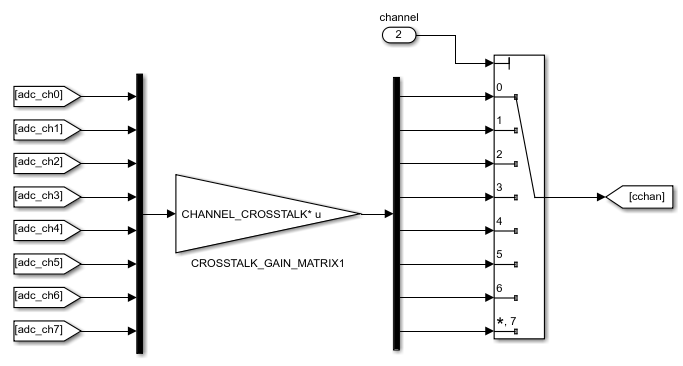
\includegraphics[scale=0.25]{pics/models/crosstalk_selector.png}
%\caption{Crosstalk injection and channel selection}
%\label{fig:crosstalksimulink}
%\end{figure}

\subsubsection{Harmonic distortion}

Harmonic distortion is artificially created in a scheme similar to one used in \cite{taheri}, consisting in taking the input signal and applying a non linear function (Figure \ref{fig:harmonixf}). The harmonics are created according to \ref{eq:harmonix} and a gain for each signal is adjusted to approximate the desired Total Harmonic Distortion (THD).

\begin{equation}
\begin{split}
sin^2(\omega t) &= \frac{1}{2}(1 - cos(2\omega t)) \\
sin^3(\omega t) &= \frac{1}{4}(3sin(\omega t) - sin(3\omega t)) \\
sin^4(\omega t) &= \frac{1}{8}(-4cos(2\omega t) + cos(4\omega t) + 3) \\
\end{split}
\label{eq:harmonix}
\end{equation}

\begin{figure}[h!]
\centering
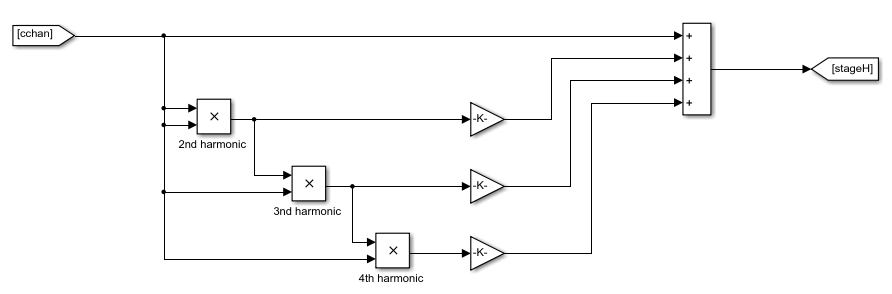
\includegraphics[scale=0.25]{pics/models/harmonix.png}
\caption{Harmonic distortion}
\label{fig:harmonixf}
\end{figure}

\subsubsection{Gain, offset and internal noise}

The final stage before quantization inserts the gain error, the offset error and adds the internal noise, modelled as a Band-Limited White Noise block. All quantities are specified in $LSB$ units and the implementation is straightforward, shown in figure \ref{fig:gainoffnoise}. 

\begin{figure}[h!]
\centering
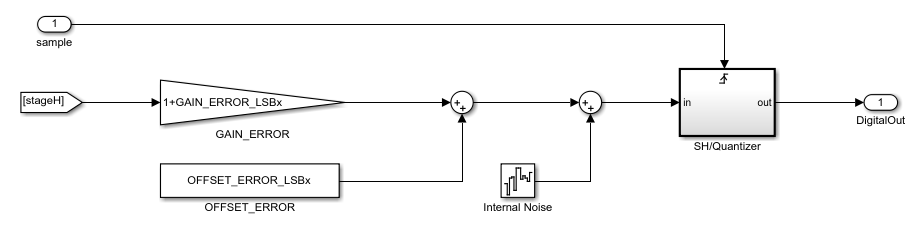
\includegraphics[scale=0.27]{pics/models/gain_off_noise.png}
\caption{Gain and offset errors and internal noise}
\label{fig:gainoffnoise}
\end{figure}

\subsubsection{Quantizer}

The strategy adopted uses a lookup table (LUT) block with interpolation disabled so the voltage read in sampling instant $kT_s$ is rounded to the nearest code. In the case of a SAR ADC, the comparator and the feedback DAC are the most significative error sources affecting code transition levels \cite{michaeli_unif}, caused by inaccuracies of the weight values for each bit $b_i$ for $i = 1, 2, \dots, N$, where N is ADC resolution. 

To generate the periodic behavior on INL, the INL vector is initialized with a sine function with low frequency (equation \ref{eq:inl_init}). The function is evaluated for $k = 1:2^N-1$. A weight value $W_0$ can be used and in this case $W_0 = 1$. For $N$ steps, a sine with double the frequency of the previous one is added to the INL vector. The obtained vector is normalized, a small amount of noise is added it is then scaled to comply with minimum and maximum values from datasheet. Since INL is found by computing the cumulative sum of DNL (equation \ref{eq:dnlcumsum}), to obtain DNL the opposite operation was used (equation \ref{eq:dnlfrominl}).

\begin{equation}
\begin{gathered}
INL_0 = W_0 * sin \left(2 \pi \frac{k}{2^N-1}\right) \\ 
INL = \sum_{n=1}^{N-1} \left(INL_{n-1} + W_n * sin\left(2^{n+1} \pi \frac{k}{2^N-1}\right)\right)
\end{gathered}
\label{eq:inl_init}
\end{equation}

\begin{equation}
INL_k = \sum_{i=1}^{k-1} DNL_i
\label{eq:dnlcumsum}
\end{equation}

\begin{equation}
DNL_k = INL_{k+1} - INL_k
\label{eq:dnlfrominl}
\end{equation}

The obtained DNL and INL values are shown on figure \ref{fig:gen_dnl_inl_x} and the values from ADS8638 datasheet are show on figure \ref{fig:real_dnl_inl_x}. The model dynamic performance parameters are summarized on table \ref{tab:adc_perf_param}.

\begin{figure}[h!]
\centering
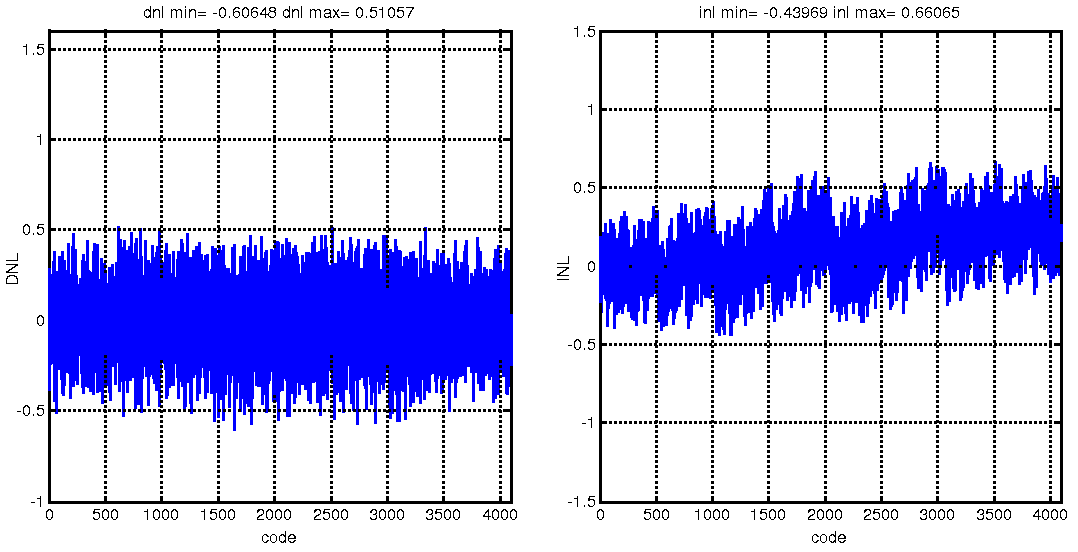
\includegraphics[scale=0.28]{pics/models/dnl_inl_2.png}
\caption{Generated DNL and INL values}
\label{fig:gen_dnl_inl_x}
\end{figure}

\begin{figure}[h!]
\centering
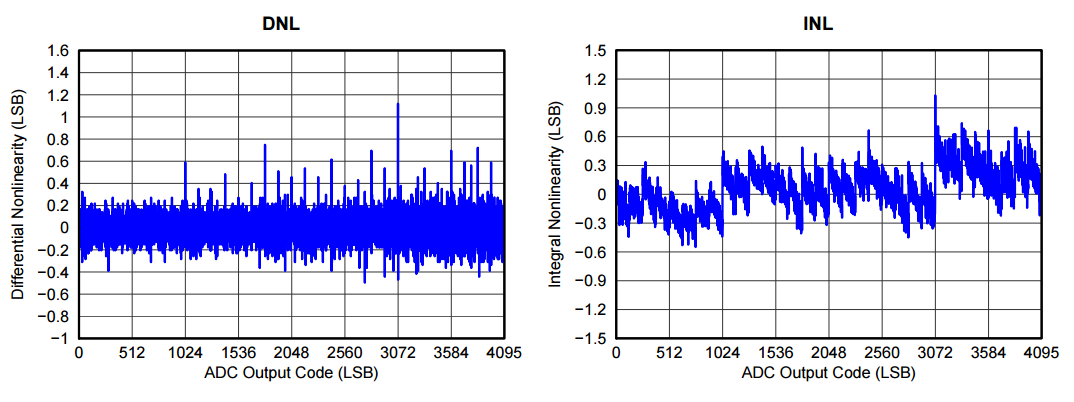
\includegraphics[scale=0.22]{pics/models/real_inl_dnl.png}
\caption{Real DNL and INL values for ADS8638 - Source: \cite{ads8638}}
\label{fig:real_dnl_inl_x}
\end{figure}

\begin{table}[h!]
\centering
\caption{ADC model dynamic performance parameters}
\label{tab:adc_perf_param}
\begin{tabular}{|c|c|c|}
\hline
Parameter & Real value & Model value \\ \hline
Signal-to-Noise ratio (SNR) & $71.8dB$ & $72.2dB$ \\ \hline
Total harmonic distortion (THD) & $-81dB$ & $-81.05dB$  \\ \hline
Signal-to-Noise-and-Distortion ratio (SINAD) & $71.3dB$ & $71.6dB$ \\ \hline
Spurious-free dynamic range (SFDR) & $-83dB$ & $-82dB$ \\ \hline
Effective number of bits (ENOB) & $11.55$ & $11.61$ \\ \hline
\end{tabular}
\end{table}	

\section{Demodulation Algorithms}

To demodulate the signal and compute the position, an LVDT of adequate range must be selected. From \cite{Ballesteros}, the excursion of the piston rod is $\pm 3.74 in$ ($\pm 95mm$). For an LVDT with stroke range of $\pm 4in$ ($ 101.6mm$) this would be about $94\%$ of the excursion leaving a small mechanical tolerance. Thus, an LVDT with stroke range equal to $\pm 5in$ ($127mm$) is selected and the rod excursion is $74.8 \%$. By convention, $L$ is the actuator length, known as pin-to-pin distance, $R$ is the horn radius and $C$ is the distance between the anchorage point in the non-moveable surface and the anchorage point in the control surface, defining the RLC triangle (Figure \ref{fig:actuator_and_surface}) \cite{Ballesteros}.

\begin{figure}[h!]
\centering
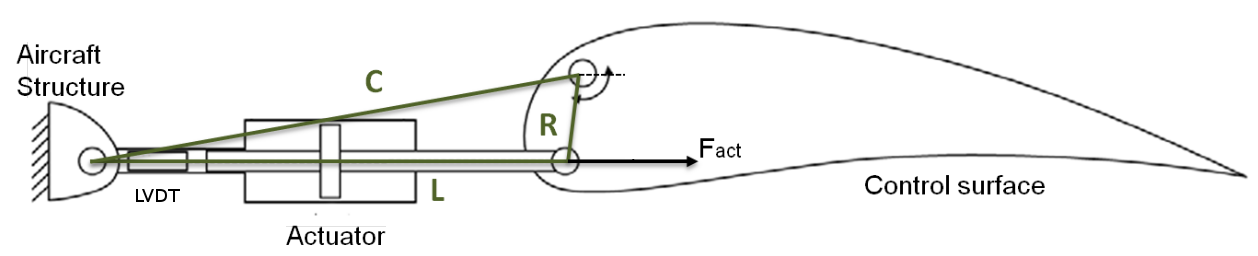
\includegraphics[scale=0.2]{pics/demodalg/actuator_and_surface.png}
\caption{Actuator, LVDT, surface and RLC triangle - Source: \cite{Ballesteros} (modified)}
\label{fig:actuator_and_surface}
\end{figure}

The variable being acquired is the piston rod position and the controlled one is the surface deflection, against which the performance of the algorithms will be evaluated. The relation between those variables is given by equation \ref{eq:pistonsurface}, where $x_p$ is the current piston rod displacement, $\theta_s$ is the surface deflection and $\beta_0$ is the angle $\widehat{RC}$ while surface is in neutral position.

\begin{equation}
\theta_s = arccos \left( \frac{R^2 + C^2 - (L_0+x_p)^2}{2RC} \right) - \beta_0
\label{eq:pistonsurface}
\end{equation}

\subsection{Peak Detector}

To obtain the peak value, the following procedure is used. The input vectors $\hat{V_a}$ and $\hat{V_b}$ are the signals from channel A and channel B respectively.

\begin{enumerate}
\item The offset value $V_{off}$ is obtained (output of the range converter when the input is zero);
\item $V_{off}$ is subtracted from both vectors and the absolute value is taken, effectively rectifying the signals;
\item The algorithm on Figure \ref{fig:peakdet0} is applied to obtain the mean peak value, where $Z_{x_t}$ is the zero crossing threshold and $Z_c$ is the counted number of samples below the threshold. The rightmost peak from each channel is discarded preventing incomplete half waves to interfere with result (Figure \ref{fig:det_peaks_uhul});
\item The mean peak values $\hat{V}_{a_{out}}$ and $\hat{V}_{b_{out}}$ are applied on equation \ref{eq:real_pos_calc} to obtain the current ratio $r_{computed}$ and then the position. For a maximum stroke ($S_{max}$) of $5in$, the maximum ratio ($r_{max}$) would be $0.5$.
\end{enumerate}


\begin{figure}[h!]
\centering
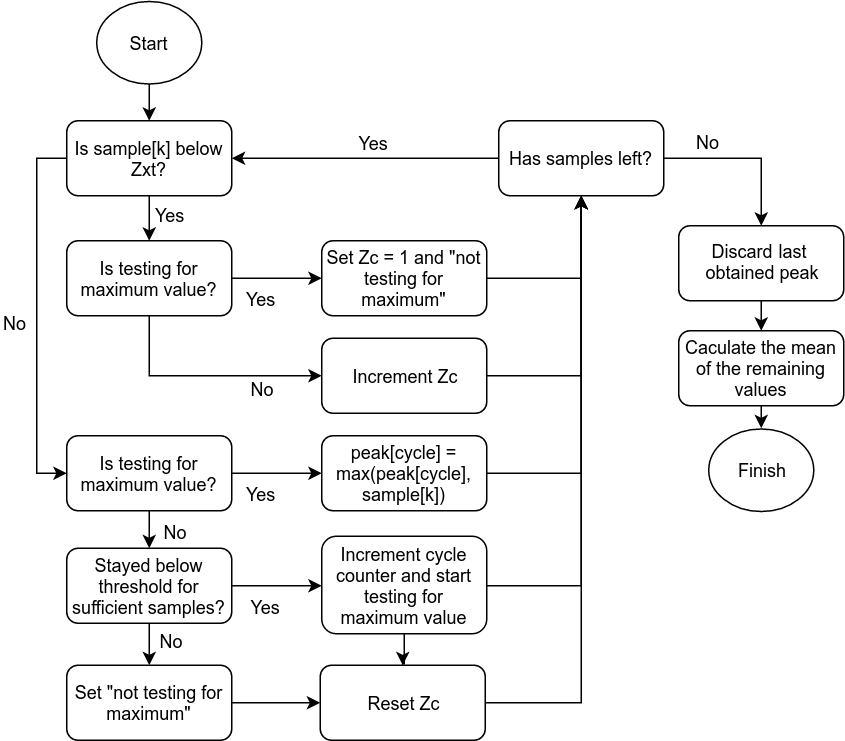
\includegraphics[scale=0.22]{pics/demodalg/peak_detection.png}
\caption{Peak detection algorithm}
\label{fig:peakdet0}
\end{figure}

\begin{figure}[h!]
\centering
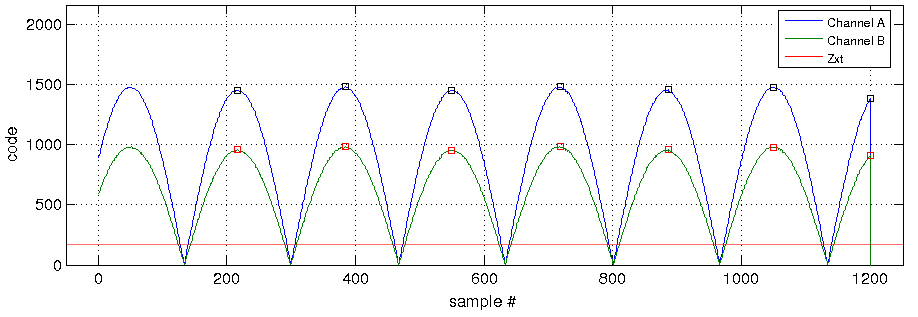
\includegraphics[scale=0.3]{pics/demodalg/detected_peaks.png}
\caption{Detected peaks}
\label{fig:det_peaks_uhul}
\end{figure}

\begin{equation}
\begin{gathered}
r_{computed} = \frac{\hat{V}_{a_{out}} - \hat{V}_{b_{out}}}{\hat{V}_{a_{out}} + \hat{V}_{b_{out}}} \\
x_{p_{computed}} = \frac{r_{computed}}{r_{max}} S_{max}
\end{gathered}
\label{eq:real_pos_calc}
\end{equation}

\subsection{Oversampling/Averaging}

Oversampling and averaging can be used to increase measurement resolution, without using a high resolution ADC. The technique improves the SNR (when white noise is concerned) and resolution at the cost of increased CPU utilization and lower throughput. To obtain the average value of the signal, the following procedure is used:

\begin{enumerate}
\item Similarly to peak detector algorithm, the signal is rectified by subtracting $V_{off}$ and taking the absolute value;
\item The first and the last zero crossings are obtained from the sampled signal delimiting a integer number of half-cycles. The points between the zero crossings are averaged for each channel;
\item The average values $\hat{V}_{a_{out}}$ and $\hat{V}_{b_{out}}$ are applied on equation \ref{eq:real_pos_calc} to obtain the current ratio $r_{computed}$ and then the position. 
\end{enumerate}

\section{Experiments}
\subsection{Steady State Error}
This experiment verifies the steady state error for a step input of $30^{\circ}$ for each algorithm in the absence of external influence. In this tests, no noise was inserted on the signal path besides the internal noise from the ADC. The gain and offset errors, correctable via calibration, are set to zero. The results are shown on Figures \ref{fig:step_steadystate_zoom} and are summarized on table \ref{tab:steady_table}.


\begin{figure}[h!]
\centering
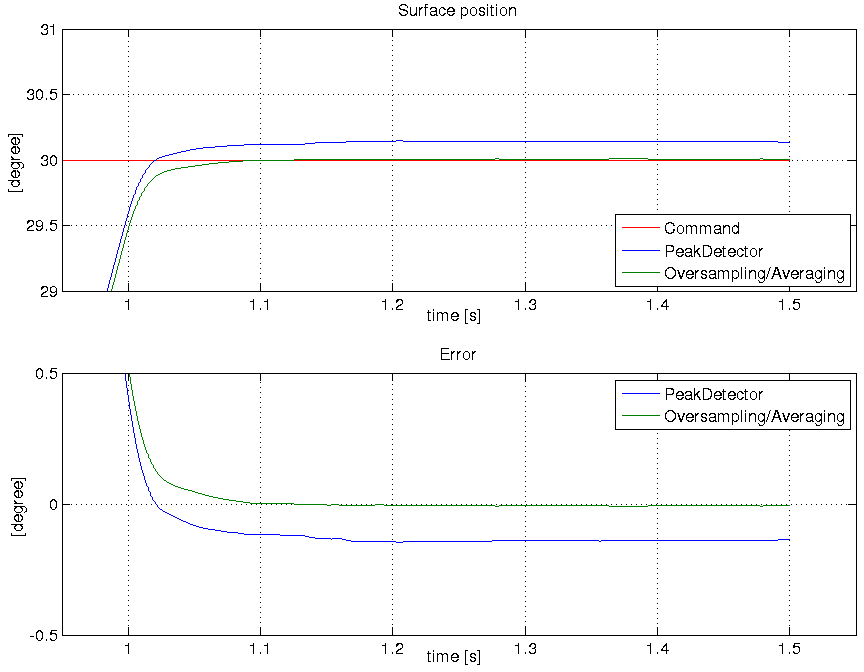
\includegraphics[scale=0.32]{pics/results/steadystate_final_zoom.png}
\caption{Step response for both algorithms in the absence of external error (zoom)}
\label{fig:step_steadystate_zoom}
\end{figure}

\begin{table}[h!]
\centering
\caption{Step input response}
\label{tab:steady_table}
\begin{tabular}{|c|c|c|c|}
\hline
Parameter 				& Expected 	& Peak Detector 	& Oversampling \\ \hline
Steady state value [${\circ}$] 		& $30.00$	& $30.14$ 	& $30.01$ \\ \hline
Steady state error [$\%$]		& $<1.00$		& $0.46$ 		& $0.02$ \\ \hline
Settling time ($1\%$) [$s$]	& -				& $0.802$ 			& $0.806$ \\ \hline
\end{tabular}
\end{table}	

\subsection{Effect of number of sampled points per cycle}

This experiment characterizes the influence the number of sampled points on each half wave in the step response of the system. Effectively, changing the number of the points is equivalent to sample at a lower frequency. To verify this effects, a point will be taken every given number of points $N$ before processing, as described by table \ref{tab:number_of_points}.

\begin{table}[h!]
\centering
\caption{Number of used points}
\label{tab:number_of_points}
\begin{tabular}{|c|c|c|}
\hline
Rule & Number of points & Effective sampling frequency \\ \hline
1/1 & 166 & $1000~kSPS$ (default) \\ \hline
1/2 & 83 & $500~kSPS$ \\ \hline
1/4 & 41 & $250~kSPS$ \\ \hline
1/8 & 20 & $125~kSPS$ \\ \hline
\end{tabular}
\end{table}	

\begin{figure}[h!]
\centering
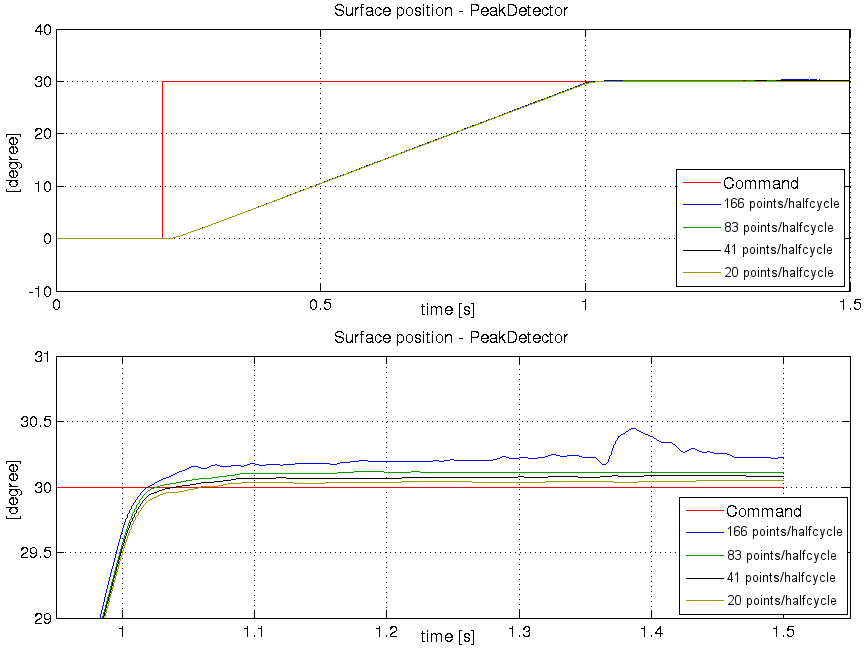
\includegraphics[scale=0.32]{pics/results/pointvar_peakdetector.png}
\caption{Effect of the number of samples on the Peak Detector algorithm}
\label{fig:pointvar_peakdetector}
\end{figure}

\begin{figure}[h!]
\centering
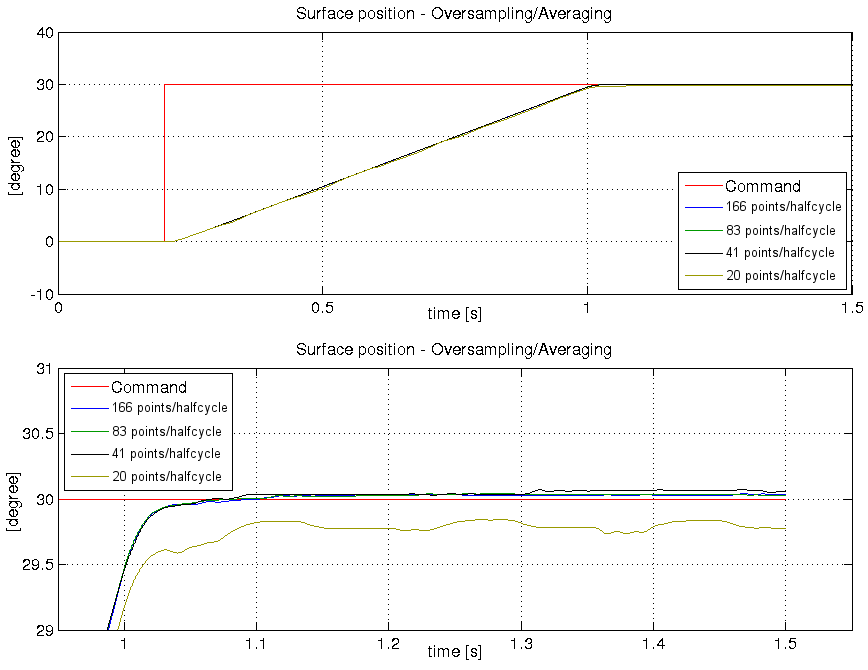
\includegraphics[scale=0.32]{pics/results/pointvar_oversampling.png}
\caption{Effect of the number of samples on the Oversampling/Averaging algorithm}
\label{fig:pointvar_oversampling}
\end{figure}

\begin{table}[h!]
\centering
\caption{Step input response - Peak Detector}
\label{tab:step_final_peakdetector}
\begin{tabular}{|c|c|c|c|c|c|}
\hline
\multirow{2}{*}{Parameter} & \multirow{2}{*}{Expected}    & \multicolumn{4}{c|}{Samples per half-cycle} \\ \cline{3-6} 
                           &                                 & 166  & 83  & 41  & 20  \\ \hline
Steady state value [$^{\circ}$]        & $30.00$	& $30.22$  & $30.11$ & $30.08$  & $30.05$   \\ \hline
Steady state error [$\%$]        & $<1.00$  		& $0.75$	   & $0.37$       & $0.27$     & $0.16$     \\ \hline
Settling time ($1\%$) [$s$]		& - 		& 	$1.218$		& $0.802$		& $0.804$ 	& $0.805$			\\ \hline
\end{tabular}
\end{table}

\begin{table}[h!]
\centering
\caption{Step input response - Oversampling/Averaging}
\label{tab:step_final_oversampling}
\begin{tabular}{|c|c|c|c|c|c|}
\hline
\multirow{2}{*}{Parameter} & \multirow{2}{*}{Expected}    & \multicolumn{4}{c|}{Samples per half-cycle} \\ \cline{3-6} 
                           &                                 & 166  & 83  & 41  & 20  \\ \hline
Steady state value [$^{\circ}$]         & $30.00$	 & $30.04$ & $30.03$ & $30.06$     & $29.78$    \\ \hline
Steady state error [$\%$]         & $<1.00$  		& $0.12$    & $0.10$       & $0.18$     &  -$0.74$    \\ \hline
Settling time ($1\%$) [$s$]		& - 		& $0.807$		& $0.806$ 		& $0.808$ 	& $0.873$			\\ \hline
\end{tabular}
\end{table}


\subsection{Tolerance to noise on input}

The following tests are intended to verify the tolerance of both algorithms to a noisy input. The same white noise signal is injected into both channels through independent current sources on each channel. The results are shown in Figures \ref{fig:noisetol_peakdetector} and \ref{fig:noisetol_oversampling} and are summarized on tables \ref{tab:step_final_noise_peakdetector} and \ref{tab:step_final_noise_oversampling}.


\begin{figure}[h!]
\centering
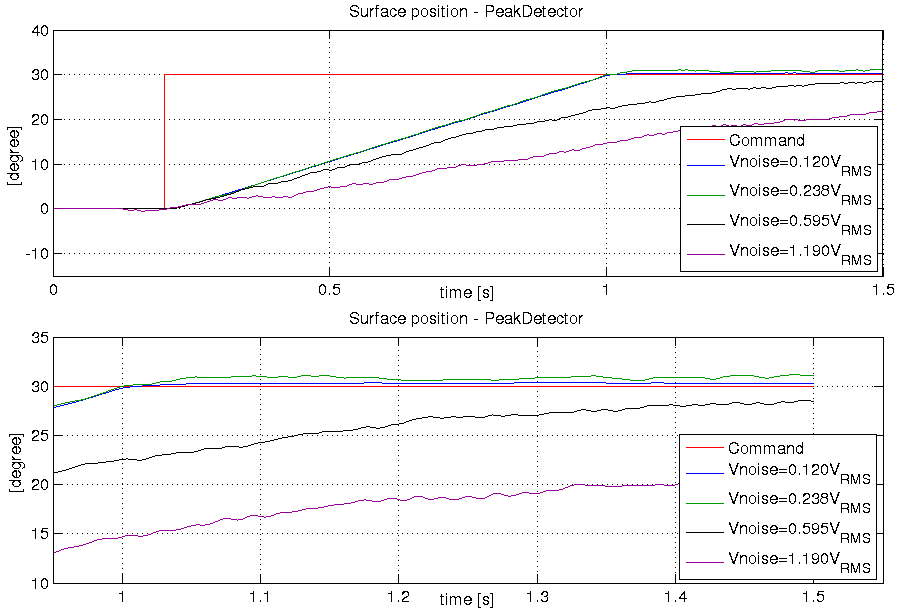
\includegraphics[scale=0.32]{pics/results/noisetol_peakdetector.png}
\caption{Effect of input noise on the Peak Detector algorithm}
\label{fig:noisetol_peakdetector}
\end{figure}

\begin{figure}[h!]
\centering
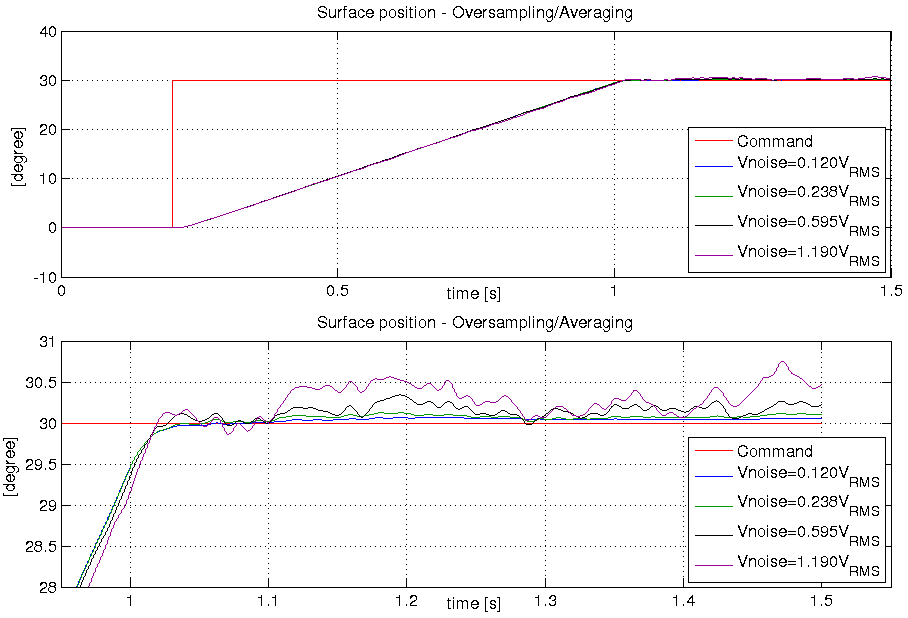
\includegraphics[scale=0.32]{pics/results/noisetol_oversampling.png}
\caption{Effect of input noise on the Oversampling/Averaging algorithm}
\label{fig:noisetol_oversampling}
\end{figure}

\begin{table}[h!]
\centering
\caption{Step input response - Peak Detector}
\label{tab:step_final_noise_peakdetector}
\begin{tabular}{|c|c|c|c|c|c|}
\hline
\multirow{2}{*}{Parameter} & \multirow{2}{*}{Expected}    & \multicolumn{4}{c|}{$V_{noise}~[V_{RMS}]$} \\ \cline{3-6} 
                           &                                 & $0.120$  & $0.238$  & $0.595$  & $1.120$  \\ \hline
Steady state value [${\circ}$]         & $30.00$	& $30.28$ & $31.05$  & $28.50$ & $21.83$ \\ \hline
Steady state error [$\%$]         & $<1.00$  		&  $0.92$       & $3.51$     & -$5.02$  & -$27.2$  \\ \hline
Settling time ($1\%$)      & - 				& $1.23$		& $-$				& $-$		& $-$			\\ \hline
\end{tabular}
\end{table}

\begin{table}[h!]
\centering
\caption{Step input response - Oversampling/Averaging}
\label{tab:step_final_noise_oversampling}
\begin{tabular}{|c|c|c|c|c|c|}
\hline
\multirow{2}{*}{Parameter} & \multirow{2}{*}{Expected}    & \multicolumn{4}{c|}{$V_{noise}~[V_{RMS}]$} \\ \cline{3-6} 
                           &                                 & $0.120$  & $0.238$  & $0.595$  & $1.120$  \\ \hline
Steady state value [${\circ}$]         & $30.00$	 &  $30.06$ & $30.11$     & $30.22$ & $30.46$ \\ \hline
Steady state error [$\%$]         & $<1.00$  		&  $0.19$       & $0.36$     &  $0.74$ & $1.55$   \\ \hline
Settling time ($1\%$) [$s$]			& - 		& $0.81$			& $0.81$		& $1.00$	& $-$			\\ \hline
\end{tabular}
\end{table}


% An example of a floating figure using the graphicx package.
% Note that \label must occur AFTER (or within) \caption.
% For figures, \caption should occur after the \includegraphics.
% Note that IEEEtran v1.7 and later has special internal code that
% is designed to preserve the operation of \label within \caption
% even when the captionsoff option is in effect. However, because
% of issues like this, it may be the safest practice to put all your
% \label just after \caption rather than within \caption{}.
%
% Reminder: the "draftcls" or "draftclsnofoot", not "draft", class
% option should be used if it is desired that the figures are to be
% displayed while in draft mode.
%
%\begin{figure}[!t]
%\centering
%\includegraphics[width=2.5in]{myfigure}
% where an .eps filename suffix will be assumed under latex, 
% and a .pdf suffix will be assumed for pdflatex; or what has been declared
% via \DeclareGraphicsExtensions.
%\caption{Simulation results for the network.}
%\label{fig_sim}
%\end{figure}

% Note that the IEEE typically puts floats only at the top, even when this
% results in a large percentage of a column being occupied by floats.


% An example of a double column floating figure using two subfigures.
% (The subfig.sty package must be loaded for this to work.)
% The subfigure \label commands are set within each subfloat command,
% and the \label for the overall figure must come after \caption.
% \hfil is used as a separator to get equal spacing.
% Watch out that the combined width of all the subfigures on a 
% line do not exceed the text width or a line break will occur.
%
%\begin{figure*}[!t]
%\centering
%\subfloat[Case I]{\includegraphics[width=2.5in]{box}%
%\label{fig_first_case}}
%\hfil
%\subfloat[Case II]{\includegraphics[width=2.5in]{box}%
%\label{fig_second_case}}
%\caption{Simulation results for the network.}
%\label{fig_sim}
%\end{figure*}
%
% Note that often IEEE papers with subfigures do not employ subfigure
% captions (using the optional argument to \subfloat[]), but instead will
% reference/describe all of them (a), (b), etc., within the main caption.
% Be aware that for subfig.sty to generate the (a), (b), etc., subfigure
% labels, the optional argument to \subfloat must be present. If a
% subcaption is not desired, just leave its contents blank,
% e.g., \subfloat[].


% An example of a floating table. Note that, for IEEE style tables, the
% \caption command should come BEFORE the table and, given that table
% captions serve much like titles, are usually capitalized except for words
% such as a, an, and, as, at, but, by, for, in, nor, of, on, or, the, to
% and up, which are usually not capitalized unless they are the first or
% last word of the caption. Table text will default to \footnotesize as
% the IEEE normally uses this smaller font for tables.
% The \label must come after \caption as always.
%
%\begin{table}[!t]
%% increase table row spacing, adjust to taste
%\renewcommand{\arraystretch}{1.3}
% if using array.sty, it might be a good idea to tweak the value of
% \extrarowheight as needed to properly center the text within the cells
%\caption{An Example of a Table}
%\label{table_example}
%\centering
%% Some packages, such as MDW tools, offer better commands for making tables
%% than the plain LaTeX2e tabular which is used here.
%\begin{tabular}{|c||c|}
%\hline
%One & Two\\
%\hline
%Three & Four\\
%\hline
%\end{tabular}
%\end{table}


% Note that the IEEE does not put floats in the very first column
% - or typically anywhere on the first page for that matter. Also,
% in-text middle ("here") positioning is typically not used, but it
% is allowed and encouraged for Computer Society conferences (but
% not Computer Society journals). Most IEEE journals/conferences use
% top floats exclusively. 
% Note that, LaTeX2e, unlike IEEE journals/conferences, places
% footnotes above bottom floats. This can be corrected via the
% \fnbelowfloat command of the stfloats package.




\section{Conclusion}
The position acquisition system was successfully modelled and integrated to the electro-hydraulic actuator model developed by \cite{Ballesteros} and the control loop was successfully closed with both demodulation strategies.

In order to evaluate the performance of the demodulation algorithms regarding steady state error, an experiment was set up minimizing the external error sources (no noise on LVDT, null gain and offset errors on ADC) and was observed that the Peak Detector responded faster, reaching the setpoint first but also presented a steady state error larger than the Oversampling/Averaging.

Regarding the variation of the number of samples, a low noise test setup caused the Peak Detector performance to improve when the number of points was reduced, since this was effectively smoothing the signal. The performance of Oversampling/Averaging degraded with reduction of the number of points reaching a steady state error greater than Peak Detector when using only $1/8$ of points. Once the noise was increased Oversampling/Averaging outperformed the Peak Detector, suggesting a higher susceptibility to noise on the latter.

The results from the noise level test confirmed that Oversampling/Averaging is more robust, being capable of resolving the rod position even with noise levels as high as $0.6V_{RMS}$ without violating the steady state error requirement of $1\%$. At noise levels as low as $0.120V_{RMS}$ the Peak Detector produced a steady state error of $0.924\%$, almost reaching the limit above mentioned.

% conference papers do not normally have an appendix


% use section* for acknowledgment
%\section*{Acknowledgment}


%The authors would like to thank...





% trigger a \newpage just before the given reference
% number - used to balance the columns on the last page
% adjust value as needed - may need to be readjusted if
% the document is modified later
%\IEEEtriggeratref{8}
% The "triggered" command can be changed if desired:
%\IEEEtriggercmd{\enlargethispage{-5in}}

% references section

% can use a bibliography generated by BibTeX as a .bbl file
% BibTeX documentation can be easily obtained at:
% http://mirror.ctan.org/biblio/bibtex/contrib/doc/
% The IEEEtran BibTeX style support page is at:
% http://www.michaelshell.org/tex/ieeetran/bibtex/
%\bibliographystyle{IEEEtran}
% argument is your BibTeX string definitions and bibliography database(s)
%\bibliography{IEEEabrv,../bib/paper}
%
% <OR> manually copy in the resultant .bbl file
% set second argument of \begin to the number of references
% (used to reserve space for the reference number labels box)
\bibliographystyle{IEEEtran}
\bibliography{IEEEabrv,references_final}


%\begin{thebibliography}{1}

%\bibitem{IEEEhowto:kopka}
%H.~Kopka and P.~W. Daly, \emph{A Guide to \LaTeX}, 3rd~ed.\hskip 1em plus
%  0.5em minus 0.4em\relax Harlow, England: Addison-Wesley, 1999.

%\end{thebibliography}

% that's all folks
\end{document}


